\documentclass[a4paper,12pt,obeyspaces,spaces,hyphens]{article}

\def \trainingtype{onsite}
\def \agendalanguage{english}

\input{agenda/preempt-rt.inc}

\usepackage{agenda}

\begin{document}

\feshowtitle

\feshowinfo

\feagendatwocolumn
{Hardware platform for practical labs}
{
  {\bf STMicroelectronics STM32MP157D Discovery Kit~1} board
  \begin{itemize}
  \item STM32MP157D (dual Cortex-A7) processor from STMicroelectronics
  \item USB powered
  \item 512 MB DDR3L RAM
  \item Gigabit Ethernet port
  \item 4 USB 2.0 host ports
  \item 1 USB-C OTG port
  \item 1 Micro SD slot
  \item On-board ST-LINK/V2-1 debugger
  \item Arduino compatible headers
  \item Audio codec, buttons, LEDs
  \end{itemize}
}
{}
{
  \begin{center}
    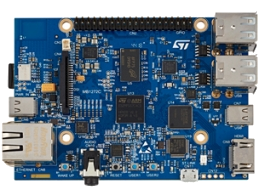
\includegraphics[width=5cm]{../slides/discovery-board-dk1/discovery-board-dk1.png}
  \end{center}
}

\section{Day 1 - Morning}

\feagendaonecolumn
{Lecture - Introduction to Real-Time behaviour and determinism}
{
  \begin{itemize}
  \item Definition of a Real-Time Operating System
  \item Specificities of multi-task systems
  \item Common locking and prioritizing patterns
  \item Overview of existing Real-Time Operating Systems
  \item Approaches to bring Real-Time capabilities to Linux
  \end{itemize}
}

\feagendatwocolumn
{Lecture - The {\em PREEMPT\_RT} patch}
{
  \begin{itemize}
  \item History and future of the {\em PREEMPT\_RT} patch
  \item Real-Time improvements from {\em PREEMPT\_RT} in mainline Linux
  \item The internals of {\em PREEMPT\_RT}
  \item Interrupt handling: threaded interrupts, softirqs
  \item Locking primitives: mutexes and spinlocks, sleeping spinlocks
  \item Preemption models
  \end{itemize}
}
{Lab - Building a mainline Linux Kernel with the {\em PREEMPT\_RT} patch}
{
  \begin{itemize}
  \item Downloading the Linux Kernel, and applying the patch
  \item Configuring the Kernel
  \item Booting the Kernel on the target hardware
 \end{itemize}
}

\section{Day 1 - Afternoon}

\feagendaonecolumn
{Lecture - Hardware configuration and limitations for Real-Time}
{
  \begin{itemize}
  \item Interrupts and deep firmware
  \item Interaction with power management features: CPU frequency
    scaling and sleep states
  \item DMA
  \end{itemize}
}

\feagendatwocolumn
{Lecture - Tools: Benchmarking, Stressing and Analyzing}
{
  \begin{itemize}
  \item Benchmarking with {\em cyclictest}
  \item System stressing with {\em stress-ng} and {\em hackbench}
  \item The Linux Kernel tracing infrastructure
  \item Latency and scheduling analysis with {\em ftrace}, {\em
      kernelshark} or {\em LTTng}
  \end{itemize}
}
{Lab - Tools: Benchmarking, Stressing and Analyzing}
{
  \begin{itemize}
  \item Usage of benchmarking and stress tools
  \item Common benchmarking techniques
  \item Benchmarking and configuring the hardware platform
  \end{itemize}
}

\section{Day 2 - Morning}

\feagendaonecolumn
{Lecture - Kernel infrastructures and configuration}
{
  \begin{itemize}
  \item Good practices when writing Linux kernel drivers
  \item Scheduling policies and priorities: {\em SCHED\_FIFO}, {\em
      SCHED\_RR}, {\em SCHED\_DEADLINE}
  \item CPU and IRQ Affinity
  \item Memory management
  \item CPU isolation with {\em isolcpus}
  \end{itemize}
}

\feagendaonecolumn
{Lecture - Real-Time Applications programming patterns}
{
  \begin{itemize}
  \item POSIX real-time API
  \item Thread management and configuration
  \item Memory management: memory allocation and memory locking, stack
  \item Locking patterns: mutexes, priority inheritance
  \item Inter-Process Communication
  \item Signaling
  \end{itemize}
}

\section{Day 2 - Afternoon}

\feagendaonecolumn
{Lab - Debugging a demo application}
{
  \begin{itemize}
  \item Make a demo userspace application deterministic
  \item Use the tracing infrastructure to identify the cause of a latency
  \item Learn how to use the POSIX API to manage threads, locking and memory
  \item Learn how to use the CPU affinities and configure the scheduling policy
  \end{itemize}
}

\feagendaonecolumn
{Questions and Answers}
{
  \begin{itemize}
  \item Questions and answers with the audience about the course topics
  \item Extra presentations if time is left, according what most
        participants are interested in.
  \end{itemize}
}

\end{document}
